\newpage

\section{Моделирование сети}

Необходимо выполнить аналитическое моделирование системы, содержащей 19 рабочих станций и сервер (ЦП и диски).\par\bigskip

Общая формализованная схема PCOD в виде сети массового обслуживания (СМО) приведена на рисунке~\ref{pic:9_1_model_general}.

\begin{figure}[h]
\center{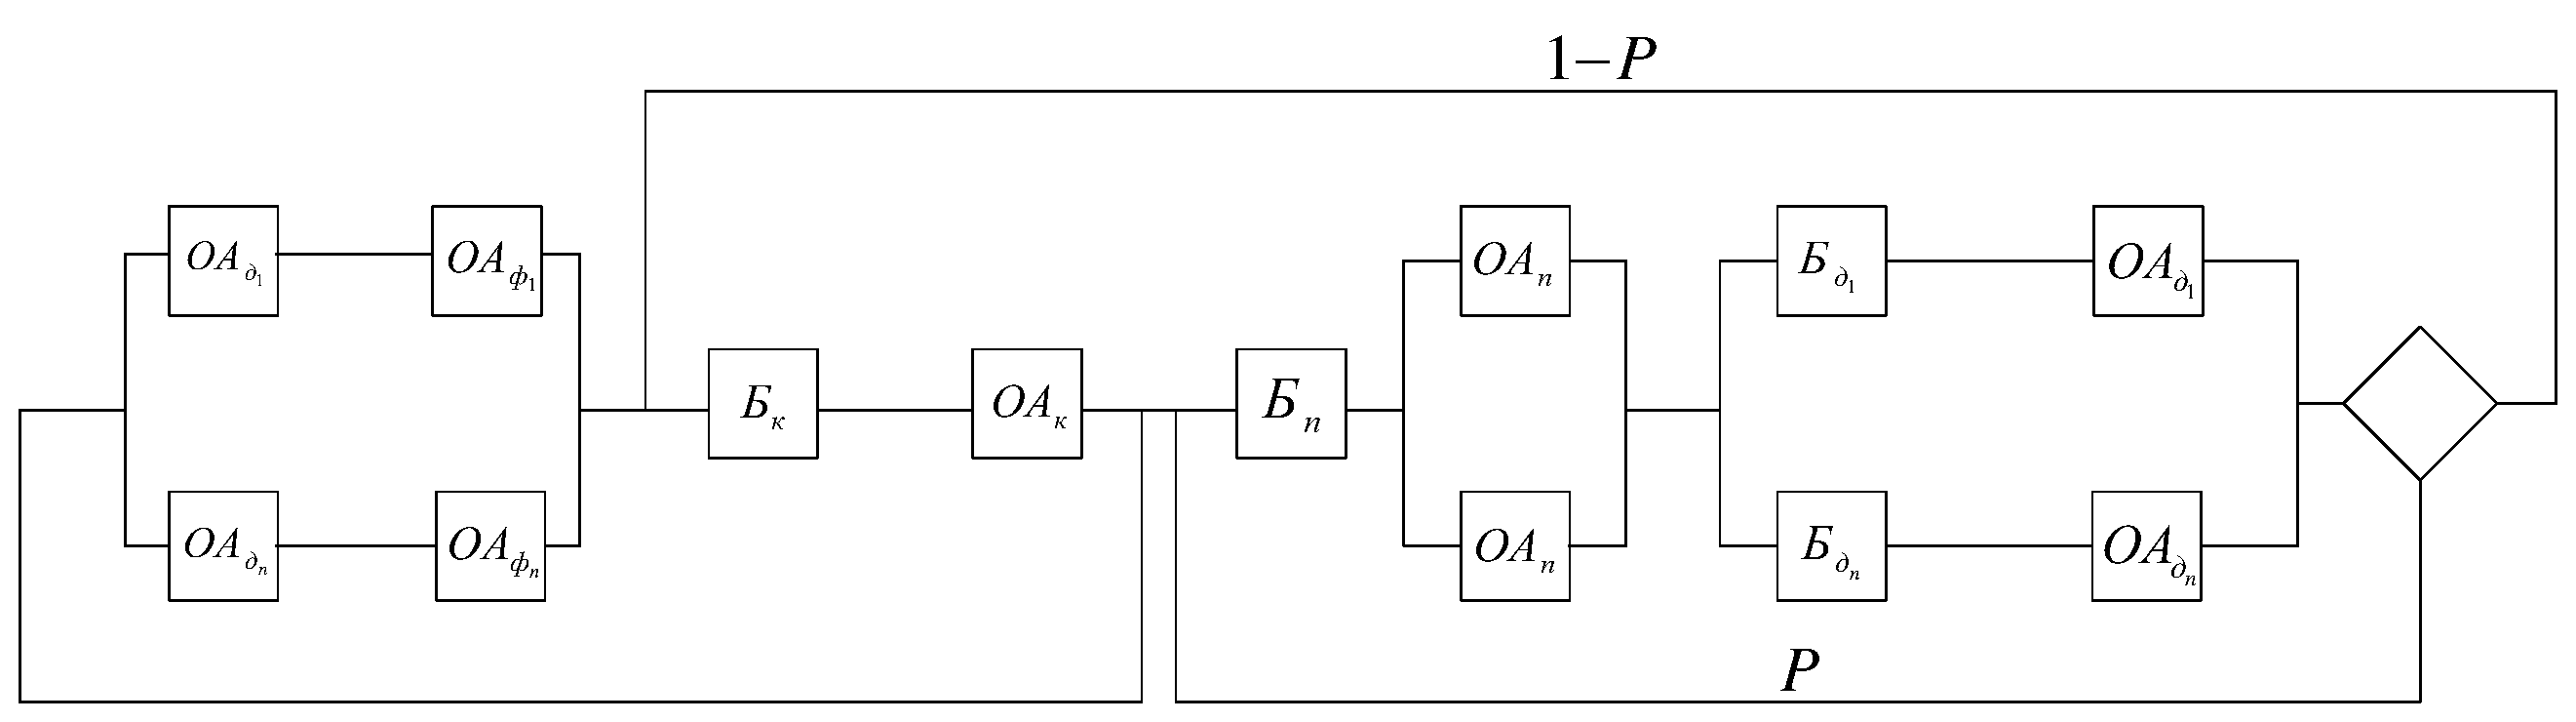
\includegraphics[width=1\linewidth]{pics/pic9_1_model_general.eps}}
\caption{Формализованная схема, содержащая ПЭВМ, канал и сервер (два ЦП и диски).}
\label{pic:9_1_model_general}
\end{figure}

В схеме используются следующие обозначения:\\
$\text{ОА}_{\text{д}_i}$ -- обслуживающий аппарат, имитирующий дообработку на $i$-той рабочей станции сети запроса от этой станции к серверу после обработки запроса на сервере;\\
$\text{ОА}_{\text{ф}_i}$ -- обслуживающий аппарат, имитирующий формирование запроса от $i$-той рабочей станции к серверу ($i = \overline{1..N}$);\\
$\text{Б}_{\text{к}}$ -- буфер, имитирующий очередь запросов к каналу;\\
$\text{ОА}_{\text{к}}$ -- обслуживающий аппарат, имитирующий задержку при передаче данных через канал;\\
$\text{Б}_{\text{п}}$ -- буфер, имитирующий очередь запросов к процессорам;\\
$\text{ОА}_{\text{п}}$ -- обслуживающие аппараты, имитирующие работу процессоров;\\
$\text{Б}_{\text{д}_i}$ -- буфер, имитирующий очередь запросов к $i$-му диску;\\
$\text{ОА}_{\text{д}_i}$ -- обслуживающий аппарат, имитирующий работу $i$-го диска;\\
$P$ -- вероятность обращения запроса к ЦП после обработки на диске. Обслуживание заявок во всех ОА подчиняется экспоненциальному закону.\par\bigskip

Формализованная схема рассматриваемой РСОД в виде CMO приведена на рисунке~\ref{pic:9_2_model_mine}.

\begin{figure}[h]
\center{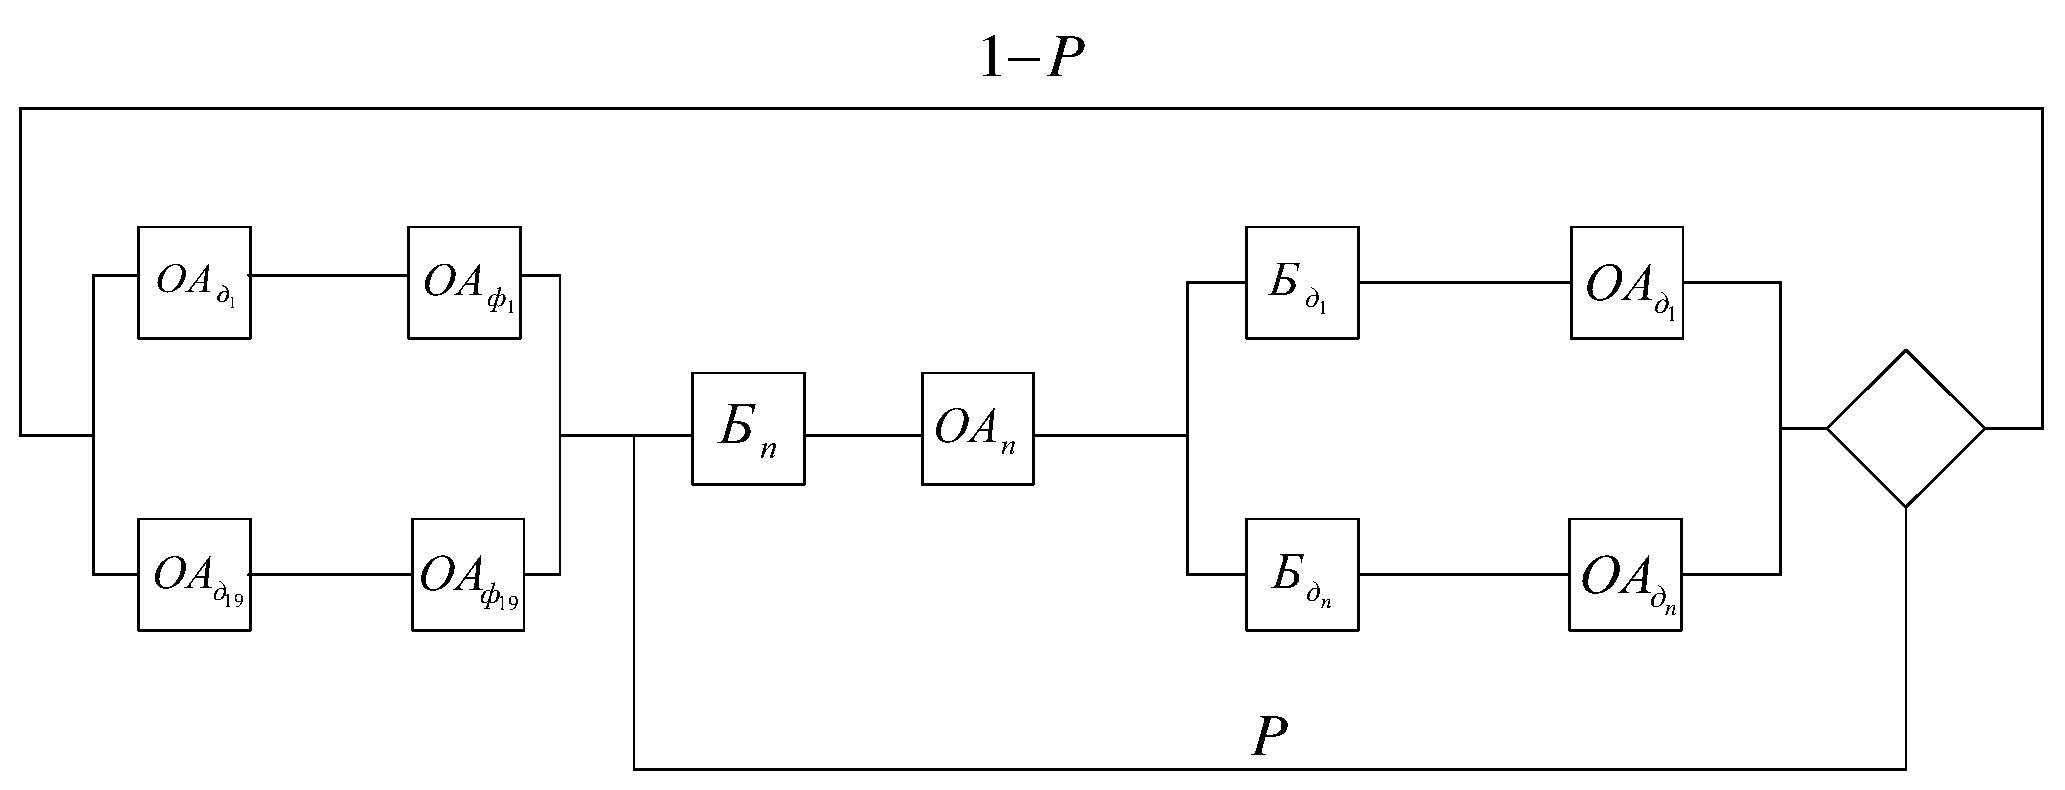
\includegraphics[width=1\linewidth]{pics/pic9_2_model_mine.eps}}
\caption{Формализованная схема рассматриваемой модели (ПЭВМ, сервер и диски).}
\label{pic:9_2_model_mine}
\end{figure}

Исходные данные модели представлены в таблице~\ref{table:in_data}.

\begin{table}[h]
\caption{Исходные данные модели}
\label{table:in_data}
\centering
 \begin{tabular}{|m{0.025\linewidth}|m{0.9\linewidth}|}
 \hline $N$ & число рабочих станций сети \\
 \hline $T_{\text{о}}$ & среднее значение времени дообработки на рабочей станции сети запроса от этой станции к базе данных на сервере \\
 \hline $T_{\text{р}}$ & среднее значение времени формирования запроса от рабочей станции сети к базе данных на сервере \\
 \hline $t_{\text{к}}$ & среднее значение времени передачи запроса по каналу \\
 \hline $\text{С}$ & число процессоров сервера \\
 \hline $t_{\text{пр}}$ & среднее значение времени обработки запроса в ЦП сервера \\
 \hline $t_{\text{д}_i}$ & среднее значение времени обработки запроса в диске сервера \\
 \hline $P_i$ & вероятность обращения запроса к $i$-му диску сервера после обработки запроса в процессоре \\
 \hline
 \end{tabular}
\end{table}

Выходные данные модели представлены в таблице~\ref{table:out_data}.

\begin{table}[h]
\caption{Выходные данные модели}
\label{table:out_data}
\centering
 \begin{tabular}{|m{0.05\linewidth}|m{0.9\linewidth}|}
 \hline $T_{\text{реак}}$ & среднее значение времени реакции системы \\
 \hline $\rho_{\text{к}}$ & коэффициент загрузки ОА, имитирующего работу канала передачи данных \\
 \hline $\rho_{\text{пр}}$ & коэффициент загрузки ОА, имитирующего работу процессора сервера \\
 \hline $\rho_{\text{д}_i}$ & коэффициент загрузки ОА, имитирующего работу i–ого диска сервера \\
 \hline
 \end{tabular}
\end{table}